\documentclass[a4paper]{jpconf}
\usepackage{amssymb,amsfonts,amsmath,mathtext,mathtools}
\usepackage{xfrac}
\usepackage{url, hyperref}
\usepackage[inline, shortlabels]{enumitem}


\newcommand{\avg}[1]{\langle{#1}\rangle}
\newcommand{\W}{\Omega}
\newcommand{\w}{\omega}
\newcommand{\nbar}{\bar n}
\newcommand{\rd}{\mathrm{d}}
\newcommand{\ddt}[1]{\frac{\rd{#1}}{\rd t}}
\newcommand{\D}{\Delta}
\newcommand{\geff}{\gamma_{eff}}

\begin{document}
	\title{Frequency domain method of the search for the electric dipole moment in a storage ring}
	\author{A E Aksentev and Y V Senichev}
	\address{Institute for Nuclear Research of the Russian Academy of Sciences, Moscow, Russia}
	\ead{a.aksentyev@inr.ru, y.senichev@inr.ru}

	\begin{abstract}
		A new method for searching for the electric dipole moment (EDM) of the deuteron and other nuclei is presented. When trying to measure the EDM in a storage ring environment, magnetic dipole moment (MDM) spin precession due to machine imperfections becomes the primary source of systematic error. The proposed method aims at providing a solution to the machine imperfection problemas well as circumventing the geometric phase error. The method is based on estimating the combined MDM~+~EDM spin precession frequency, in which the MDM contribution is due only to field imperfections. The MDM term is canceled in the final statistic by  adding frequency estimates from cycles with counter-circulating beams. Spin precession rate depends on the particle's effective Lorentz factor; the proposed method's core feature is a procedure for equalizing the effective Lorentz factors of the clockwise and counter-clockwise circulating beams, thus enabling the cancelation.
	\end{abstract}

\section{Introduction}
One of the essential problems of modern physics is the baryon asymmetry of the universe, which indicates the prevalence of matter over antimatter.~\cite{Canetti} In addition, the cosmic detectors PAMELA and AMS, whose purpose is to search for antimatter, have yet to find a significant amount of it in the universe.~\cite{Aguilar} A new idea claiming that one of the reasons for the baryon asymmetry is the breaking of CP invariance emerged soon after its discovery. A. Sakharov established the conditions for baryogenesis in 1967.~\cite{Sakharov} Many theories beyond the Standard Model (SM) have been proposed -- all of them new physics theories -- that are able to remove the difficulties encountered in the SM but have yet to be proven in experiments. One of the possible signatures for the breaking of CP invariance is the existence of non-vanishing electric dipole moments (EDM) of elementary particles.

\section{Machine imperfection MDM spin precession}
Tilting of the accelerator optical elements about the beam axis induces a non-zero average radial magnetic field, which causes an EDM-faking MDM precession. 

We have simulated the machine imperfection precession rate $\W_{MDM}$ for the frozen spin (FS) lattice depicted in Figure~\ref{fig:Lattice}. The lattice utilizes cylindrical E+B field spin rotators in the arc sections in order to effect the FS condition. Imperfections were simulated via rotations of the E+B elements about the optical axis by normally-distributed angles $\Theta_{tilt}\sim N(0,10^{-4})$~rad. The standard deviation of $10^{-4}$~rad was chosen as an estimate of a practically-achievable element alignment error level. Analytical estimates~\cite{Senichev:FDM} show, that at this level, the machine imperfection $\W_{MDM}$ should be expected in the range of 50 to 100 rad/sec, assuming an $n=100$ element lattice.


\begin{figure}[h]\centering
	\begin{minipage}{.5\linewidth}
		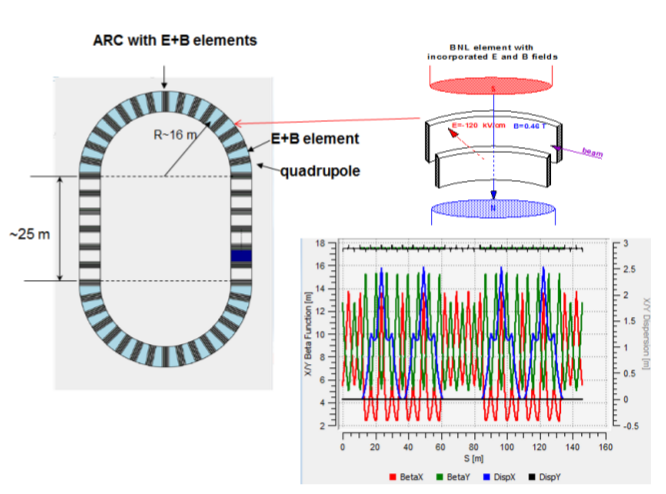
\includegraphics[width=\linewidth]{Figures/BNL}
		\caption{Frozen spin lattice with cylindrical E+B field spin rotators inserted into the arc sections.\label{fig:Lattice}}
	\end{minipage}\hspace*{2mm}
	\begin{minipage}{.5\linewidth}
		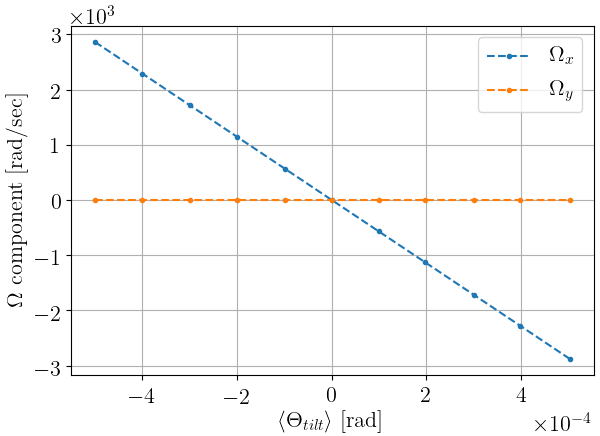
\includegraphics[width=\linewidth]{Figures/linearity_test_shifting_gauss_freq}
		\caption{Spin precession frequency components vs mean E+B element tilt angle.\label{fig:MDM_vs_tilt}}
	\end{minipage}
\end{figure}

%\begin{figure}[h]\centering
%	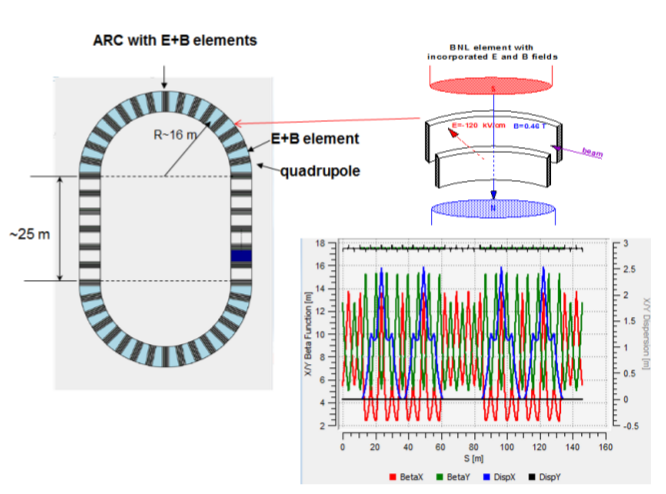
\includegraphics[width=.7\linewidth]{Figures/BNL}\hspace{3mm}%
%	\begin{minipage}[b]{.2\linewidth}\caption{Frozen spin lattice with cylindrical E+B field spin rotators inserted into the arc sections.\label{fig:Lattice}}
%	\end{minipage}
%\end{figure}

Simulation results are presented in Figure~\ref{fig:MDM_vs_tilt}. One can observe that at $\avg{\Theta_{tilt}}=10^{-4}$~rad the radial component of $\W_{MDM}$ is approximately 500~rad/sec. 
Since $\sigma[\avg{\Theta_{tilt}}]~=~\sigma[\Theta_{tilt}]/\sqrt{n} = 10^{-4}/\sqrt{100} = 10^{-5}$~rad. The dependence in Figure~\ref{fig:MDM_vs_tilt} is linear, hence the probability of observing $\W_{MDM}\le 50$~rad/sec is 68\%, $\W_{MDM}\le 100$~rad/sec is 95\%, and $50\le\W_{MDM}\le100$~rad/sec with a 27\% probability.

%\begin{figure}[h]\centering
%	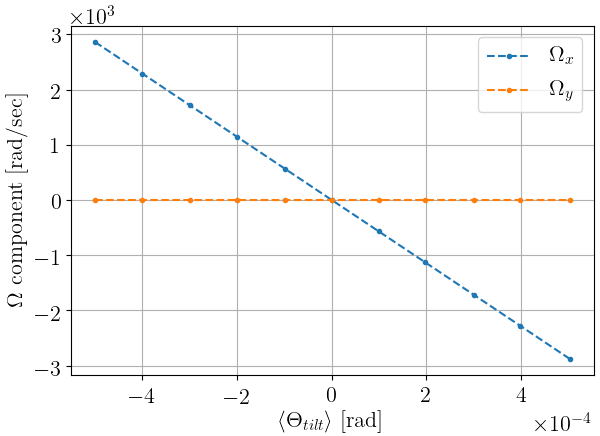
\includegraphics[width=.55\linewidth]{Figures/linearity_test_shifting_gauss_freq}\hspace{3mm}%
%	\begin{minipage}{.35\linewidth}\caption{Spin precession frequency components vs mean E+B element tilt angle.\label{fig:MDM_vs_tilt}}
%	\end{minipage}
%\end{figure}

\section{BNL and Koop Method}
The idea of searching for the electric dipole moment (EDM) of the proton and the deuteron using polarized beams in a storage ring is based on the ``frozen'' spin method and was originally proposed at Brookhaven National Laboratory (BNL)~\cite{Farley}.

The orientation of the spin in 3d space is determined by three frequency projections of spin precession $\W_x, \W_y, \W_z$ due to magnetic dipole moment and electric dipole moment:
\begin{equation}\label{eq:Omega}
\W=\sqrt{\left(\W_{EDM}+\W_x\right)^2+\W_y^2+\W_z^2}	
\end{equation}

The main idea of the ``frozen'' spin concept is to create such a configuration of external fields that in an ideal storage ring without element imperfectios the spin orientation changes only due to the presence of an electric dipole moment $\W_{EDM}$. 
In a non-ideal storage ring when $\W_x\neq0, \W_y\neq0, \W_z\neq0$, the spin changes in accordance with:
\begin{equation}\label{eq:Sy-oscillation}
	\tilde{S}_y = \sqrt{\left(\frac{\W_y\W_z}{\W^2}\right)^2 + \left(\frac{\W_x + \W_{EDM}}{\W}\right)^2}\cdot \sin(\W\cdot t + \phi).
\end{equation}

In the BNL method the deviation of the spin vector in the vertical plane is measured, that is, the amplitude of the changing part of the signal  during a long time (approx. 1000 sec). 

Expecting it at the level of $\tilde{S}_y\approx10^{-6}$~rad after $t\approx1000$~sec and assuming that it is necessary to correct all misalignments to such a magnitude $\W_x,\W_y, \W_z\ll\W_{EDM}$ that the contribution will be determined only by the EDM signal. However, if the frequencies in all three planes are of the same order and close, but not equal to zero, then the invariant spin axis is completely undefined, that is, in each element of the ring the spin rotates around the most pronounced axis with an indefinite amplitude. The effect of mixing the frequencies with the frequency of the EDM occurs, which, despite the use of two beams moving in opposite directions clockwise (CW) and counter-clockwise (CCW), eliminates the certainty of the measurement. This effect is called the ``geometric phase'' and it remains unresolved in the BNL method. Besides, in the BNL method, the procedure of restoring the magnetic field after changing polarity is not defined. All these unsolved problems do not allow considering the BNL method as feasible.

Another method developed by Ivan Koop~\cite{Koop2015} has a fundamental difference from the BNL method. In his concept of colliding or co-rotating ion beams I. Koop suggests to store two ion beams, circulating with different velocities, where one beam is polarized and its EDM is measured using the `frozen spin' method, and the second beam, which is unpolarized, is used as a co-magnetometer, sensitive to the radial component of the ring's magnetic field. Having studied Koop’s method, we have certain remarks. 

Firstly, the author is using two beams, and one of them -- the polarized beam -- is used to measure the spin precession frequency, obviously using a polarimeter. However, he does not pay attention to the fact that the energy of a polarized beam determines the efficiency of interaction with the polarimeter target. For example, let's consider the first example from Table 2 in~\cite{Koop2015}, where the energy of a polarized proton beam is 16~MeV. If we compare the figure of merit at this energy and the energy at which it is supposed to conduct experiments on measuring the EDM, namely 230~MeV, then the number of useful events at 16~MeV will be 4 orders of magnitude lower. This means that the required number of events will require time proportional to this factor.

Secondly, the author claims that in his method the spin coherence time can be several orders of magnitude higher due to the introduction of a transverse magnetic field. And this is partly correct, since a relatively fast spin oscillation in the vertical plane periodically changes the sign of horizontal decoherence, therefore it limits the value of horizontal decoherence within its growth during the half-period of vertical oscillation. However, now we are interested in spin decoherence in the vertical plane, since the success of measuring the frequency of spin precession for determining the EDM is determined by the preservation of polarization in the vertical plane. But vertical decoherence is completely determined by the spread of the effective value of the Lorentz factor~\cite{Senichev:FDM}. Therefore the vertical decoherence is also corrected using sextupoles~\cite[p.~40]{Aksentev:Thesis} and it remains at the same level as the horizontal decoherence in the BNL method. Thus, this method has no advantages in this matter as well.

Now we need to discuss the most important idea of Koop’s ``spin wheel'' method. Starting the presentation of the method, the author makes an estimate of the contribution of the average radial magnetic field at a level of $10^{-13}$~Gauss, which produces a mimic effect comparable with the EDM at the level $d=10^{-29}~e\cdot$cm. Then they write that such a small magnetic field could be detected only via measurement of the separation of mean orbits of two beams in the vertical direction making reference to the report of D. Kawall.~\cite{Kawall} According to Kawall, the accompanying beam orbit splitting is on the order of $10^{-12}$~m. Then it is suggested that the EDM contribution to the measured spin precession rate can be extracted just by comparing runs with positive ($+\Delta$)  and negative ($-\Delta$) separation of mean orbits:
\begin{equation*}
	\W_{EDM} = \frac{\W_x(+\Delta) + \W_x(-\Delta)}{2}.
\end{equation*}

Here the author supposes two tings:
\begin{enumerate*}[(1)] 
\item that they can measure the average value of the orbit with an accuracy of $10^{-12}$~m using SQUIDs and \label{itm:Koop-assumption-1}
\item that the MDM spin precession frequency is completely determined by the average orbit, hence $\W_{MDM}(+\Delta) = -\W_{MDM}(-\Delta)$. \label{itm:Koop-assumption-2}
\end{enumerate*}

We disagree with assumption~\ref{itm:Koop-assumption-1} on the grounds that
\begin{enumerate*}[(a)]
	\item such an orbit displacement measurement accuracy has never been shown experimentally, and
	\item even if it were possible, the estimates in~\cite{Kawall} presuppose weak focusing in the vertical plane and a 0.1 betatron oscillation phase advance, which excludes the possibility of correcting spin decoherence in such a lattice.
\end{enumerate*}

We believe asumption~\ref{itm:Koop-assumption-2} to be false because the spin precession frequency of a bunched beam in the presence of an RF field depends on the beam orbit length, but not the average orbit shift $\Delta$.

\section{Frequency Domain Method}
\subsection{Geometric phase error}
Geometric phase (GP) error is the accumulation of spin rotation in the vertical $y-z$ plane caused by non-commuting rotations in the horizontal $x-z$ and transverse vertical $x-y$ planes.~\cite[p.~23]{AGS-proposal-deuteron} Formulated in the frequency domain language, it is a result of a lack of a definite direction of the spin precession axis. 

In our Frequency Domain Method~\cite{Senichev:FDM} we are going to use only the measurement of the spin precession frequency and with the accuracy that already has been experimentally verified.~\cite{Bagdasarian} Unlike the BNL method, we measure not the amplitude $\tilde S_y$, but the frequency $\W$ of the spin oscillations~\eqref{eq:Sy-oscillation}.

Our goal in minimizing the GP effect is to make the $\W_{EDM}$ contribution to $\W$ much larger than that of $\W_y$ and $\W_z$. The first of these frequencies is minimized by fulfilling the FS condition in the horizontal plane: $\W_y\approx0$ (precision to which the FS condition needs to be fulfilled is estimated below). The $\W_z$ frequency is minimized by using an additional longitudinal solenoid on the beam line. 

The condition that needs to be fulfilled for the minimization of the GP error is as follows:~\cite[p.~4]{Senichev:FDM}
\begin{equation}\label{eq:GP-minimization-condition}
\W_{EDM} > \frac{\W_y^2 + \W_z^2}{2\W_x}.
\end{equation}
Since we expect the $\W_x$ in the range of 50 to 100~rad/sec, it follows that making $\W_y,\W_z~<~10^{-3}$~rad/sec is sufficient to minimize the GP error to below the $\W_{EDM}$ value. Note that the solution of the GP problem does not require knowledge of the precise values of $\W_y$ and $\W_z$; they just have to be small.

\subsection{EDM estimator statistic}
Since the measured frequency $\W = \W_{MDM} + \W_{EDM}$ includes a contribution due to the MDM, one has to find a way to eliminate the $\W_{MDM}$ term from the final $\hat\W_{EDM}$ estimator. 

In the proposed methodology, non-spurious $\W_{MDM}$ is generated only by the radial magnetic fields induced by accelerator element tilts about the optical axis. Therefore, by reversing the polarity of the guide field one also reverses the sign of $\W_{MDM}$. The EDM estimator is constructed as a sum of positive (beam circulates clockwise) and negative (counter-clockwise) polarity cycles' angular momentum estimates:
\begin{align}
\W^{\pm} &= \pm \W_{MDM}^\pm + \W_{EDM},\\
\hat\W_{EDM} &= \frac12\left[\hat\W^+ + \hat\W^-\right] \notag\\
&= \W_{EDM} + \frac{1}{\sqrt{2}}\cdot\sigma_{MDM} + \epsilon,	\label{eq:EDM-estimator}
\end{align}
where
$\sigma_{MDM}$ is  the statistical (model parameter estimate) error, and the difference between the two cycles' MDM spin precession rates $\epsilon~=~\frac12\left(\W_{MDM}^+~-~\W_{MDM}^-\right)$ is the  systematic error term.

\subsection{Effective Lorentz factor}
In order to minimize systematic error $\epsilon$, one needs a way to keep $\W_{MDM}$ constant across multiple runs.

The obvious way of trying to precisely reproduce the guiding field is inefficient for two major reasons:
\begin{enumerate*}[(1)]
	\item standard magnetic field measurement methods do not yield sufficient precision;
	\item the lattice might not be symmetric enough, in terms of spin dynamics, with respect to reversal of the beam circulation direction.
\end{enumerate*}
Hence, we propose a different variable for calibration.

We note that the number of spin revolutions per turn (spin tune $\nu_s$) depends on the particle's  equilibrium-level energy, expressed by the Lorentz factor $\gamma$:
\begin{align}\label{eq:spin_tune_vs_gamma}
\nu_s^B &= G\gamma, \tag{magnetic field}\\
\nu_s^E &= \frac{G+1}{\gamma} - G\gamma. \tag{electric field}
\end{align}

Not all beam particles in a bunch are characterized by the same $\gamma$. A particle involved in betatron
motion will have a longer orbit, and as a direct consequence of the phase stability principle,
in an accelerating structure utilizing an RF cavity, its equilibrium energy level 
must increase.

The effective Lorentz factor $\geff = \gamma_s + \beta_s^2\gamma_s\cdot\delta_{eq}$ is a generalization of the regular Lorentz factor $\gamma_s$ (of the reference particle) accounting for betatron motion-related orbit lengthening $(\Delta L/L)_\beta$ and non-linearity of the momentum compaction factor $\alpha = \alpha_0 + \alpha_1\delta$; there $\delta=\Delta p/p_s$, and the equilibrium level momentum shift~\cite{Senichev:FDM, Senichev:IPAC13}
\begin{equation*}\label{eq:equ-delta-shift}
	\Delta\delta_{eq} = \frac{\gamma_s^2}{\gamma_s^2\alpha_0-1}\left[\frac{\delta_m^2}{2}\left(\alpha_1 - \frac{\alpha_0}{\gamma_s^2}+ \frac{1}{\gamma_s^4}\right) + \left(\frac{\Delta L}{L}\right)_\beta\right].
\end{equation*}
In the equation above, $\delta_m$ is the amplitude of synchrotron oscillations.

It has been shown in~\cite[p.~56]{Aksentev:Thesis} that a particle's spin tune can be described by a univariate function; we associate the argument of that function with the effective Lorentz factor. Consequently, spin-vectors of two particles characterized by the same value of the effective Lorentz factor precess as the same rate.

Therefore, if the CW and CCW beam centroids' have equal $\geff$, we can expect the MDM components of the spin precession angular velocities to be equal as well.

\subsubsection{Calibration of the ELF}
Calibration of the effective Lorentz factor is done via observing spin precession in the closed orbit plane. For that purpose, a special transverse spin rotator element is used in order to suppress the vertical plane precession.  Using the fact that $\nu_s$ is an injective function of $\geff$, it follows that there exists a unique value $\geff^0$, at which the polarization vector is frozen with respect to the beam's momentum vector in the horizontal plane, i.e. $\nu_s=0$ in the rest frame. Since the tilt of the spin precession axis is the same for the CW and CCW beams,  
\[
\lim_{\nu_s^+ - \nu_s^- \to 0} \W_{MDM}^+ - \W_{MDM}^- = 0,
\]
and hence $\epsilon$ in equation~\eqref{eq:EDM-estimator} is removed.

\section{Statistical precision}
Spin precession frequency is estimated via non-linear fit of a constant-parameter harmonic function to polarization data. However, perturbations to the spin dynamics, caused by, for example, betatron motion, introduce a mismatch between the fit model and the data, and hence a model specification systematic error. This problem has been analyzed,~\cite{Aksentev:IPAC19:SMP} with the conclusion that this systematic error is negligible.

Effective measurement cycle length cannot exceed three times the polarization lifetime $\tau_d$,~\cite{Stats} where $\tau_d$ is the time during which beam polarization decreases by a factor of $e$.

Simulation shows~\cite{Stats} the possibility of reaching a statistical error $\sigma[\hat\W]=8\cdot10^{-7}$~rad/sec in one measurement cycle (at $\tau_d = 721$~sec, cycle length $10^3$~sec), and $\sigma[\avg{\hat\W}]=5\cdot10^{-9}$~rad/sec in one year of measurement (at 70\% accelerator time load). This should suffice to achieve an EDM estimate precision level of $10^{-29}~e\cdot$cm.

\section{Conclusion}
In this paper we described the frequency domain method for searching for the deuteron EDM in an imperfect storage ring. The method differs from~\cite{Farley, AGS-proposal-deuteron} in that frequency of oscillations, as opposed to vertical polarization component value, is used to infer the value of the EDM. This enables us to have a definite orientation of the spin precession axis, and hence avoid the geometrical phase error. 
The proposed method differs from~\cite{Koop2015} in that no other variable except frequency needs to be measured. The concept of the \textit{effective} Lorentz factor has been described, which we believe to be essential in analyzing the particle spin dynamics in storage ring.

\section*{References}
\begin{thebibliography}{4}
	\bibitem{Canetti}
	Canetti L, Drewes M and Shaposhninkov M 2012 Matter and antimatter in the universe \textit{New J. Phys.} \textbf{14} 095012
	\bibitem{Aguilar}
	Aguilar M \textit{et al} 2013 \textit{Phys. Rev. Lett.} \textbf{110} 141102
	\bibitem{Sakharov}
	Sakharov A 1967 \textit{J. Exp. Theor. Phys.} \textbf{5} 24-6
	\bibitem{Senichev:FDM}
	Senichev Y, Aksentev A, Ivanov A and Valetov E  2017 Frequency domain method of the search for
	the deuteron electric dipole moment in a storage ring with imperfections \textit{Preprint} arxiv:1711.06512 [physics.acc-ph]
%	\url{https://arxiv.org/abs/1711.06512}.
	\bibitem{Farley}
	Farley F J M, Jungmann K, Miller J P, Morse W M, Orlov Y F, Roberts B L, Semertzidis Y K, Silenko A and Stephenson E J 2004 \textit{Phys. Rev. Lett.} \textbf{93} 052001
	\bibitem{Koop2015}
	Koop I A 2015 \textit{Phys. Scr.} \textbf{2015} 014034
	\bibitem{Aksentev:Thesis}
	Aksentev A 2019 2D Frozen spin method of searching for the deuteron EDM in a storage ring \textit{Preprint} thesiscommons.org/cn4x3
%	\url{http://collaborations.fz-juelich.de/ikp/jedi/public_files/theses/dissertation.pdf}
	\bibitem{Kawall}
	Kawall D 2011 Beam position monitors with SQUIDs for the
	pEDM experiment, Report at 485 WE-Heraeus EDM
	Seminar (Bad Honnef)
	\bibitem{AGS-proposal-deuteron}
	Anastassopoulos D \textit{et al} 2008 AGS proposal: search for a permanent electric dipole moment of the deuteron ucleus at e $10^{-29}~e\cdot$cm level \textit{Brookhaven National Laboratory Report}
	\bibitem{Bagdasarian}
	Bagdasarian Z \textit{et al} 2014 \textit{Phys. Rev. ST Accel. Beams} \textbf{17} 052803
	\bibitem{Senichev:IPAC13}
	Senichev Y, Maier R, Zyuzin D and Kulabukhova N 2013 \textit{Proc. 4th International Particle Accelerator Conference (IPAC'13)} 12--17 May 2013 Shanghai, China 2579-81
	\bibitem{Aksentev:IPAC19:SMP}
	Aksentev A, Senichev Y 2019 Spin Motion Perturbation Effect on the EDM Statistic
	in the Frequency Domain Method \textit{Proc. 10th International Particle Accelerator Conference (IPAC'19)} 19--24 May 2019 Melbourne, Australia pp 861-3
%	\url{https://ipac2019.vrws.de/papers/mopts011.pdf}
	\bibitem{Stats}
	Aksentev A E, Senichev Y V 2017 \textit{J Phys: Conf Ser.} \textbf{941} 012083
%	\url{https://iopscience.iop.org/article/10.1088/1742-6596/941/1/012083}
	
\end{thebibliography}

\end{document}